\chapter{T3a --- Muchos cuerpos: trayectorias cuánticas}
\label{ch:t3a}

\ideacentral{T3a valida que la \emph{dinámica de relajación} de muchos cuerpos
---el escenario donde el QMpE es físicamente rico y el Liouvilliano explícito de
T1 es imposible--- se puede simular con trayectorias estocásticas (memoria $2^N$
en vez de $4^N$), reproduciendo la ecuación maestra exacta dentro del error
estadístico $M^{-1/2}$ y con escalado \emph{casi ideal}. Es decir: la simulación
sobre la que se observaría y explotaría el efecto es correcta y escalable a
tamaños inaccesibles a T1.}

\section{Marco teórico}

Cuando $4^N$ excede la memoria disponible, el Liouvilliano explícito deja de ser
viable. El método de \textbf{trayectorias cuánticas} (Monte Carlo wavefunction;
Dalibard--Castin--Mølmer; ver Daley, \emph{Adv. Phys.} \textbf{63}, 77, 2014)
reemplaza la propagación del operador densidad $\rho\in\mathbb{C}^{d\times d}$ por
la de $M$ \emph{vectores de estado} estocásticos $\ket{\psi}\in\mathbb{C}^d$, y
recupera
\begin{equation}
    \rho_t = \mathbb{E}\big[\ket{\psi_t}\!\bra{\psi_t}\big]
           \approx \frac{1}{M}\sum_{m=1}^{M}\ket{\psi_t^{(m)}}\!\bra{\psi_t^{(m)}}.
\end{equation}
La memoria pasa de $d^2=4^N$ a $d=2^N$, lo que permite alcanzar $N$ inviables para
la ecuación maestra. El error estadístico del promedio decae como $M^{-1/2}$.

\section{Método numérico: saltos cuánticos}

Cada trayectoria evoluciona con el Hamiltoniano efectivo no hermítico
$H_{\mathrm{eff}} = H - \tfrac{i}{2}\sum_\mu L_\mu^\dagger L_\mu$. En cada paso $dt$:
\begin{align}
    \ket{\psi'} &= \ket{\psi} - i\,dt\,H_{\mathrm{eff}}\ket{\psi},
    & \delta p &= 1 - \langle\psi'|\psi'\rangle.
\end{align}
Se extrae $r\sim U[0,1]$: si $r<\delta p$ ocurre un \emph{salto}, se elige el canal
$\mu$ con probabilidad $\propto\langle\psi|L_\mu^\dagger L_\mu|\psi\rangle$ y se
aplica $\ket{\psi}\to L_\mu\ket{\psi}/\|L_\mu\ket{\psi}\|$; si no, se normaliza la
propagación determinista $\ket{\psi}\to\ket{\psi'}/\|\psi'\|$.

\paragraph{Acción matrix-free para muchos cuerpos.}
En el núcleo C++ (\texttt{T3/T3a\_trajectories/cpp/qtraj\_mpi.cpp}) ni $H$ ni los
$L_\mu$ se almacenan: la acción sobre $\ket{\psi}$ se calcula localmente,
explotando la estructura de la cadena de Ising \cref{eq:ising}. La parte diagonal
($-J\sum Z_iZ_{i+1}$ y $\sum_\mu L_\mu^\dagger L_\mu$) es un signo por estado de la
base; la parte $-h\sum_i X_i$ conecta cada estado con sus $N$ vecinos por
volteo de un bit; los saltos $\sigma_\pm^i$ son operaciones locales. El coste por
paso es $\mathcal{O}(N\,d)$, sin matrices.

\section{Implementación serial}

La referencia serial (\texttt{python/qtraj.py}, función \texttt{evolve\_serial})
promedia $M$ trayectorias en un solo proceso. Cada trayectoria usa un generador
de números aleatorios con semilla propia, garantizando independencia y
reproducibilidad.

\section{Justificación de la paralelización}

Las trayectorias son \emph{independientes}: este es el caso \emph{embarrassingly
parallel} por excelencia. La única comunicación es la reducción final del
observable promediado. Se explotan dos niveles:
\begin{itemize}
  \item \textbf{MPI} (internodo): cada rango simula $M/K$ trayectorias y el
  resultado se combina con \texttt{MPI\_Reduce}.
  \item \textbf{OpenMP} (intranodo): dentro de cada rango, las trayectorias
  locales se reparten entre hilos, cada uno con su acumulador y su RNG.
\end{itemize}
En Python, la versión \texttt{evolve\_parallel} usa \texttt{multiprocessing} como
equivalente de memoria compartida. Al no haber acoplamiento secuencial (a
diferencia de T1), se espera escalado casi ideal.

\section{Comparación y resultados}

\subsection{Convergencia y validación}

La \cref{fig:t3aconv} valida el método contra la ecuación maestra exacta (TLS): el
error RMS del promedio decae con pendiente log--log $-0.488$, en excelente acuerdo
con la ley teórica $M^{-1/2}$. La validación cruzada del núcleo C++ contra el
oráculo denso (Ising $N=3$, $M=20\,000$) da un error máximo de $8\times10^{-3}$,
dentro del error estadístico esperado.

\begin{figure}[t]
\centering
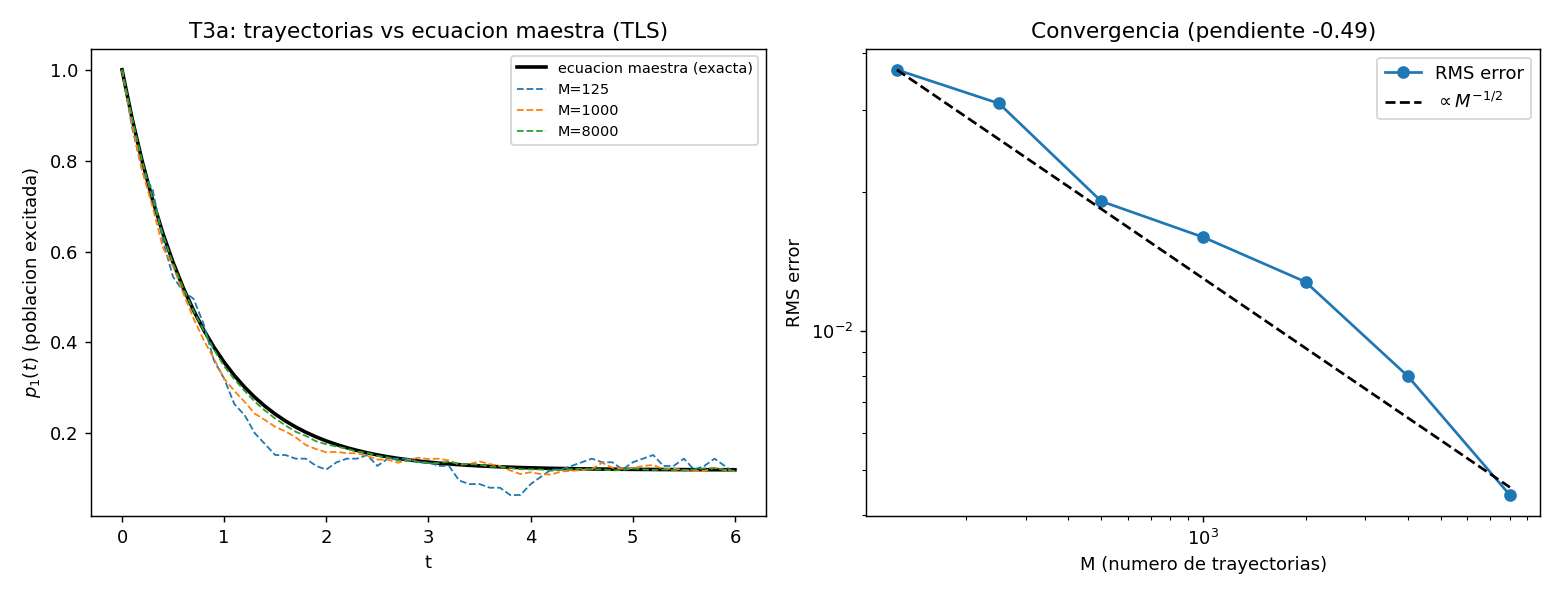
\includegraphics[width=\textwidth]{figures/t3a_convergence.png}
\caption{T3a: (izq.) población excitada del TLS, trayectorias frente a la ecuación
maestra exacta; (der.) error RMS frente a $M$, con pendiente $-0.488\approx-1/2$.}
\label{fig:t3aconv}
\end{figure}

\subsection{Escalado paralelo}

La \cref{tab:t3ascaling} y la \cref{fig:t3ascaling} muestran el escalado del núcleo
C++ sobre Ising $N=10$ ($d=1024$; el Liouvilliano denso sería $4^{10}\approx10^6$
de dimensión, imposible). El escalado es \emph{casi ideal} y prácticamente idéntico
para OpenMP y MPI, como corresponde a un problema embarrassingly parallel. El
contraste con T1 (\cref{tab:t1scaling}) es la lección central de Sistemas
Distribuidos: la estructura del acoplamiento del algoritmo determina su
escalabilidad.

\begin{table}[h]
\centering
\caption{T3a: speedup de las trayectorias distribuidas (Ising $N=10$, $d=1024$,
$M=1024$).}
\label{tab:t3ascaling}
\begin{tabular}{ccc}
\toprule
workers & OpenMP & MPI \\
\midrule
2 & $1.95\times$ & $1.96\times$ \\
4 & $3.72\times$ & $3.73\times$ \\
8 & $4.77\times$ & $4.64\times$ \\
\bottomrule
\end{tabular}
\end{table}

\begin{figure}[t]
\centering
\begin{subfigure}{0.49\textwidth}
  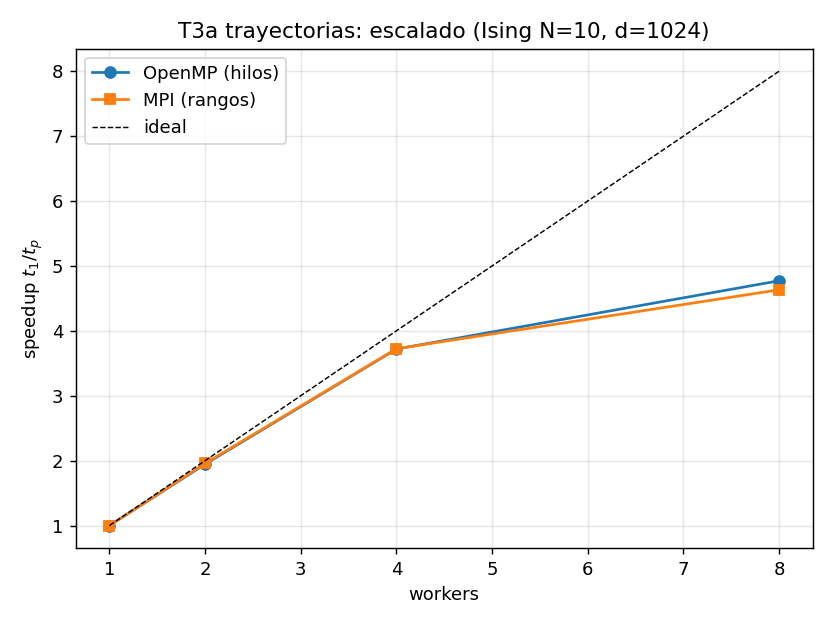
\includegraphics[width=\textwidth]{figures/t3a_scaling.png}
\end{subfigure}\hfill
\begin{subfigure}{0.49\textwidth}
  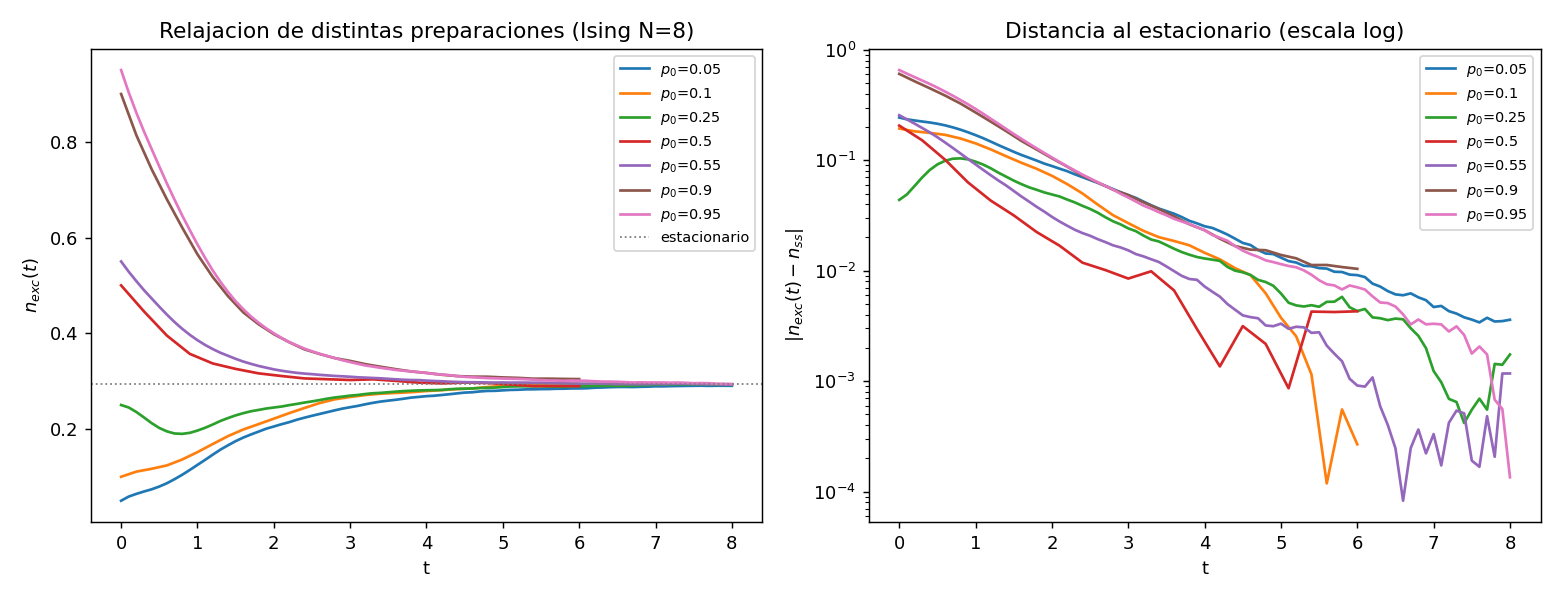
\includegraphics[width=\textwidth]{figures/t3a_curves.png}
\end{subfigure}
\caption{T3a: (izq.) escalado casi ideal de OpenMP y MPI; (der.) relajación de la
densidad de excitación de distintas preparaciones $p_0$ de la cadena de Ising
$N=8$ hacia un estado estacionario común.}
\label{fig:t3ascaling}
\end{figure}

Además, en Python el promedio con \texttt{multiprocessing} sobre el TLS alcanza un
speedup de $4.6\times$ (M=4000) frente al serial, confirmando el mismo patrón en
memoria compartida.
